\chapter{Controlled Spatial Transformation With Deterministic Mapping Function}
\section{Introduction}


 In chapter 2, we elaborated on the details of the patient-adaptive ECG classification framework. An important part of this methodology is to design a \textit{personalized classifier} with a \textit{deviation analysis module}. The performance of the \textit{deviation analysis module} depends on the geometry of different classes of data samples in the feature space. In chapter 3, we proposed a novel spatial transformation method based on MOPSO to  achieve a desired symmetry in the transformed feature space to boost the performance of the deviation analysis module. This methodology enables us to further process the normal samples and identify fuzzy states between the normal and abnormal states. However, the proposed method uses an iterative optimization which may have high computational complexity. In this chapter, we introduce another deterministic spatial transformation method to model the fuzzy state of samples with a more tractable and analytical solution. %These two methods share a common concept of modeling the intermediate states from annotated normal to abnormal state. 

 
While the aforementioned method in Chapter 3 yields the desired capacity of predicting upcoming abnormalities, the interpretation of the mechanisms of the system is not straightforward and easily tractable, thus it is not easily generalizable to a broader range of applications in the biomedical signal processing. The main objective of this chapter is to develop a deterministic transformation with a stronger prediction power based on a controlled spatial topology studied in Chapter 3. In this method, we further optimize the topology and spatial geometry of the clusters in the feature space by reducing the within-cluster variance after the spatial transformation. As shown in Fig. \ref{fig:topo2}, through this improvement, the performance of the personalized classifier in terms of prediction accuracy can be further enhanced with the proposed method.
 
%Having analyzed the symmetric encircled topology in the previous chapter, we proposed a novel spatial transformation based predictive modeling system to assist cardiologist take advanced therapeutic Interventions. In this method, we further optimize the topology and spatial geometry of clusters in the feature space by reducing the within cluster variance after spatial transformation. As shown in \ref{fig:topo2}, through this improvement, the predicting accuracy of personal classifier can be further improved.
\begin{figure}[t]
\centering
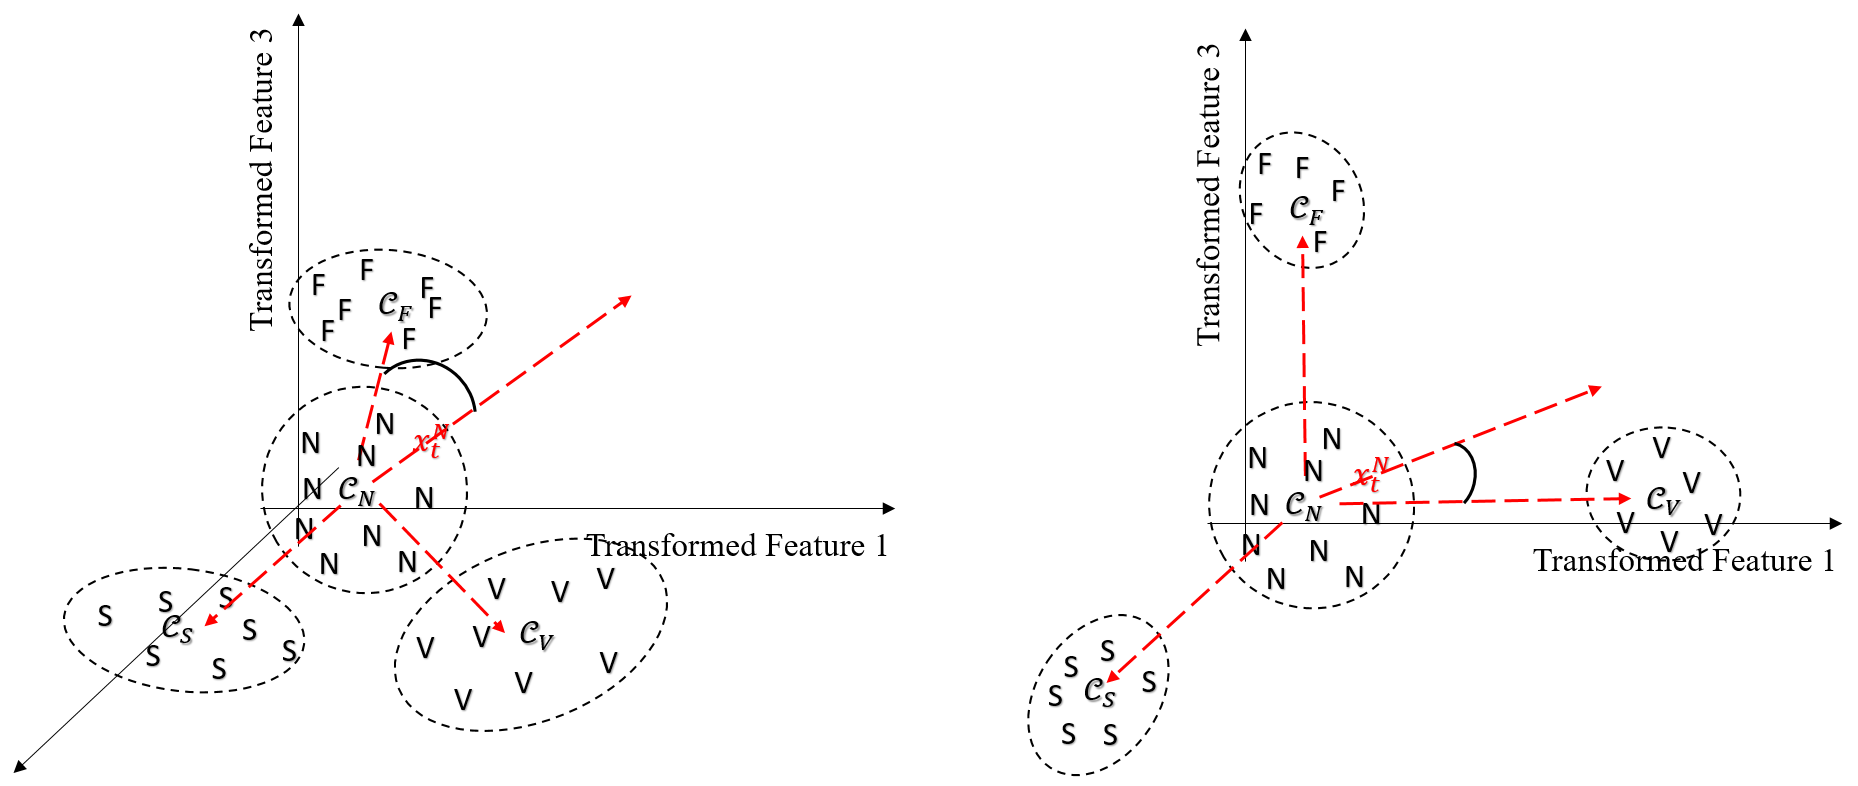
\includegraphics[scale=.42]{Fig/topo2.png}
\caption{Left: illustration of the clustering topology in the \textcolor{black}{transformed feature space without reducing the within-cluster variance}; % transformed with a simple mapping function;  
Right: illustration of the clustering topology in the \textcolor{black}{feature space transformed with the optimized mapping function, which reduces the within-cluster variance.}}%\textcolor{red}{Razi: it is not clear what you mean here by simple, is it unoptimized, why not just saying the original space before transmission !}}
\label{fig:topo2}
\end{figure}

\section{Hyper-Spherical Coordinates}

In the previous chapter, the spatial transformation module is implemented with a polynomial kernel function and a heuristic optimization method. The system performance has been proven to be promising. In addition to the general drawbacks of heuristic method, it is not straightforward to select an appropriate base kernel as the core of spatial mapping function due to the high variety of kernel functions. % and the limitation of dimensionality.

In order to address this issue, a novel deterministic spatial mapping function is proposed in this chapter based on \textit{hyper-spherical} coordinates\cite{nsphere}. Since hyper-spherical coordinates consist of angles and radius, these parameters in both original feature space and the desired target space are used to determine the mapping function.


The hyper-spherical coordinate system (n-dimensional spherical coordinate system) and its mapping to the \textit{Cartesian} coordinate system are first introduced in \cite{nsphere}. If $\mathbf{x}$ is a sample vector in 
a $n$-dimensional feature space, with its Cartesian coordinates $(\xi_1,~\xi_2~... \xi_n)$, then its corresponding hyper-spherical coordinates can be obtained through Eq.\ref{eq:cart2sph}, which is originally derived through its reverse mapping (Eq.\ref{eq:sph2cart}) using equation: $\sin(\arccos(x)) = \sqrt{1-x^2}$.



\begin{align}
\label{eq:cart2sph}
\nonumber
r      &= \sqrt{{\xi_n}^2 + {\xi_{n-1}}^2 + \cdots + {\xi_2}^2 + {\xi_1}^2} \\
\nonumber
\theta_1 &= \arccos \frac{\xi_{1}}{\sqrt{{\xi_n}^2+{\xi_{n-1}}^2+\cdots+{\xi_1}^2}} \\
\nonumber
 \theta_2 &= \arccos \frac{\xi_{2}}{\sqrt{{\xi_n}^2+{\xi_{n-1}}^2+\cdots+{\xi_2}^2}} \\
\nonumber
        &\vdots\\
\nonumber
 \theta_{n-2} &=\arccos \frac{\xi_{n-2}}{\sqrt{{\xi_n}^2+{\xi_{n-1}}^2+{\xi_{n-2}}^2}} \\
 \theta_{n-1} &= 
 \begin{cases}
     \arccos \frac{\xi_{n-1}}{\sqrt{{\xi_n}^2+{\xi_{n-1}}^2}} & \xi_n\geq 0 \\
     - \arccos \frac{\xi_{n-1}}{\sqrt{{\xi_n}^2+{\xi_{n-1}}^2}} & \xi_n < 0
 \end{cases} 
\end{align}


\begin{align}
\label{eq:sph2cart}
\nonumber
\xi_1 &= r \cos(\theta_1) \\
%\xi_j &= r \cos(\theta_j)\prod_{k=1}^{j-1}\sin(\theta_k)\\
\nonumber
\xi_2 &= r \sin(\theta_1) \cos(\theta_2) \\
\nonumber
\xi_3 &= r \sin(\theta_1) \sin(\theta_2) \cos(\theta_3) \\
\nonumber
    &\vdots\\
\nonumber
\xi_{n-1} &= r \sin(\theta_1) \cdots \sin(\theta_{n-2}) \cos(\theta_{n-1}) \\
\xi_n &= r \sin(\theta_1) \cdots \sin(\theta_{n-2}) \sin(\theta_{n-1}),
\end{align}


where $0\leq \theta_j\leq\pi,~j=1,\dots ,n-2$; $0\leq \theta_{n-1}\leq 2 \pi$; $0\leq r<\infty$
 
 
\section{Orthogonalization}

To simplify the algorithm, in this chapter, the topology of clusters in the feature space is approximated by their centroid locations, \textcolor{black}{denoted by $\mathbf{c}_N^k, \mathbf{c}_{\mathcal{V}}, \mathbf{c}_{\mathcal{S}}, \mathbf{c}_{\mathcal{F}}$, respectively for the normal cluster and the three abnormality clusters of type $V$, $S$, and $F$.} Furthermore, as we assume that the samples with fuzzy states deviate from the normal cluster to a specific abnormality cluster, the spatial topology stays unchanged if the normal centroid is simply translated to the origin of the Cartesian coordinate system. The clustering topology in the original feature space can be equivalently represented by the following matrix with three row vectors:

\begin{align}
\mathcal{C} = 
\begin{bmatrix}
\mathbf{c}_{\mathcal{V}} - \mathbf{c}_N^k \\
\mathbf{c}_{\mathcal{S}} - \mathbf{c}_N^k \\
\mathbf{c}_{\mathcal{F}} - \mathbf{c}_N^k
\end{bmatrix} = 
\begin{bmatrix}
\mathbf{v}_{\mathcal{VN}} \\
\mathbf{v}_{\mathcal{SN}} \\
\mathbf{v}_{\mathcal{FN}}
%\mathbf{v}_{\mathcal{VN}} \\
%\mathbf{v}_{\mathcal{SN}} \\
%\mathbf{v}_{\mathcal{FN}}
\end{bmatrix}
\end{align}
%\textcolor{red}{RZ: I used lower case $v$ for vectors, which is more consistent with other definitions. Capital letter are more commonly used for matrices.}

As shown in Fig. \ref{fig:topo2}, in order to improve the performance of the personalized classifier and to avoid ambiguity in quantifying the deviations to different abnormality classes, a topology with a maximum separation between the three vectors of $\mathcal{C}$ is preferred. To achieve a lower computational complexity in higher order dimensions, the algorithm aims at transforming vectors in $\mathcal{C}$ to orthogonal vectors using a deterministic function. This approach not only simplifies the transformation derivations, it also ensures a full symmetry among abnormality clusters. As such, the problem reduces to finding a transformation that maps a set of vectors to a set of orthogonal vectors in the same space. Therefore, we can use the popular method of \textit{Gram-Schmidt} orthogonalization method \textcolor{black}{explained} in \cite{Gram-schmidth1, Gram-schmidth2}. Hence, in the first step of this stage, the three row vectors of $\mathcal{C}$ representing the centroids of the three abnormality clusters are fed to the orthogonalization process as follows:
\begin{align}
\mathcal{C}^{\perp}= \text{Gram-Schmidt}(\mathcal{C})
=
\begin{bmatrix}
\mathbf{v}_{\mathcal{VN}}^{\perp} \\
\mathbf{v}_{\mathcal{SN}}^{\perp} \\
\mathbf{v}_{\mathcal{FN}}^{\perp},
\end{bmatrix}
\end{align}

where $\mathcal{C}^{\perp}$ is the matrix of orthogonalized vectors in the Cartesian coordinate system. The hyper-spherical coordinates $\mathcal{C}^{\perp}_{*}$ of these orthogonalized vectors are calculated subsequently using Eq.\ref{eq:cart2sph}. After this step, the orthogonalized vectors in the hyper-spherical coordinate system are obtained as formulated in Eq. \ref{eq:c_ortho}. The $j^{th}$ angular dimension denoted as  $\theta_{j}^{\perp}$ and the radius is noted as $r^{\perp}$.%, which reveals the angular change from original vectors to the ideal orthogonal vectors, are calculated subsequently using Eq.\ref{eq:cart2sph}.

\begin{align}
\label{eq:c_ortho}
\mathcal{C}^{\perp}_{*} =
\begin{bmatrix}
    r_{\mathcal{VN}}^{\perp} & \theta_{1_{\mathcal{VN}}}^{\perp} & \dots  & \theta_{{n-1}_{\mathcal{VN}}}^{\perp} \\
    r_{\mathcal{SN}}^{\perp} & \theta_{1_{\mathcal{SN}}}^{\perp} & \dots  & \theta_{{n-1}_{\mathcal{SN}}}^{\perp} \\
%    \vdots & \vdots & \ddots & \vdots \\
	r_{\mathcal{FN}}^{\perp} & \theta_{1_{\mathcal{FN}}}^{\perp} & \dots  & \theta_{{n-1}_{\mathcal{FN}}}^{\perp} \\
\end{bmatrix}
\end{align}


\section{Spatial Mapping Function}
After obtaining the original hyper-spherical coordinates of $[\mathbf{v}_{\mathcal{VN}},~\mathbf{v}_{\mathcal{SN}},~\mathbf{v}_{\mathcal{FN}}]^T$ and the orthogonalized hyper-spherical coordinates $[\mathbf{v}_{\mathcal{VN}}^{\perp},~\mathbf{v}_{\mathcal{SN}}^{\perp},~\mathbf{v}_{\mathcal{FN}}^{\perp}]^T$, the goal is to design a mapping function $\mathbf{F}: \mathbf{R}^n \to \mathbf{R}^n$ from the original coordinates to the orthogonal ones which exhibit the desired clustering topology, \textcolor{black}{such that Eq. \ref{eq:constraints} holds.}

In the Gram-Schmidt algorithm, the very first vector serves as a reference vector and remains unchanged in the orthogonalization process, namely $\mathbf{v}_{\mathcal{VN}} = \mathbf{v}_{\mathcal{VN}}^{\perp}$. Therefore the mapping function $\mathbf{F}$ shall satisfy the following equations:

\begin{align}
\label{eq:constraints}
\begin{aligned}
%\mathbf{F}(0) &= 0 &~\\
\mathbf{F}(\mathbf{v}_{\mathcal{SN}} - \mathbf{v}_{\mathcal{VN}}) &= \mathbf{v}_{\mathcal{SN}}^{\perp} - \mathbf{v}_{\mathcal{VN}}^{\perp} &= \mathbf{v}_{\mathcal{SN}}^{\perp} - \mathbf{v}_{\mathcal{VN}}\\
\mathbf{F}(\mathbf{v}_{\mathcal{FN}} - \mathbf{v}_{\mathcal{VN}}) &= \mathbf{v}_{\mathcal{FN}}^{\perp} - \mathbf{v}_{\mathcal{VN}}^{\perp} &= \mathbf{v}_{\mathcal{FN}}^{\perp} - \mathbf{v}_{\mathcal{VN}}
\end{aligned}
\end{align}

Furthermore, since the orthogonality of vectors is independent to their radii $r$, we only need to design $\mathbf{F}$ for the $n-1$ angular dimensions ($\theta_1,\dots,\theta_{n-1}$), and the coordinate $r$ remains unchanged after the mapping. Consequently, the function $\mathbf{F}$ can be decomposed into $n-1$ functions: $f_i: \mathbf{R}\to \mathbf{R},~i=1\dots n-1$ with constraints in Eq.\ref{eq:constraints} as well as two additional extreme points defining the range of input and output values. %  \textcolor{red}{RZ: this part is not clear: and boundary constraints of angular dimensions, specified in Equi XXX: add equations for clarity.} 
%In order to standardize $f_i$ for all angular dimensions, $\theta_i, ~i=1\dots n-2$ are proportionally scaled to the range between $(0,2\pi)$.
We use the notation $\mathbf{v}_{\mathcal{SN}} - \mathbf{v}_{\mathcal{VN}} = \Delta_{\mathcal{SV}}$ and denote the the $i^{th}$ angular dimension of $\Delta_{\mathcal{SV}}$ as $\delta_{i_{{\mathcal{SV}}}}$. We use similar notations for the other dimensions, (e.g. $\mathbf{v}_{\mathcal{FN}} - \mathbf{v}_{\mathcal{VN}}$). %Hence for each angular dimension $i, i = 1,\dots, n-2$, $\delta_{i_{{\mathcal{SV}}}}$ and $\delta_{i_{{\mathcal{FV}}}}$ are both within the range of $(-\pi,\pi)$
Hence for each angular dimension $i$, $f_i$ is determined by ($\delta_{i_{{\mathcal{SV}}}}$,$\delta^{\perp}_{i_{{\mathcal{SV}}}}$) and ($\delta_{i_{{\mathcal{FV}}}}$,$\delta^{\perp}_{i_{{\mathcal{FV}}}}$), \textcolor{black}{along with the two \textit{extreme boundary points} defining the domain and range of the functions.}



 %boundary constraints of angular dimensions. \textcolor{red}{RZ: Neads a little bit of clarification: by boundary constraints, do you mean the domain(input range) of the functions?. 2-Do you mean that $f_i$ should be designed such that it maps the two points () and () in the original space into points () and () in the target space?}
%if $f_i$ is to be depicted with a curve in 2-D plane, this curve will 4 points: (0,0), ($\delta_{i_{{\mathcal{SV}}}}$,$\delta^{\perp}_{i_{{\mathcal{SV}}}}$), ($\delta_{i_{{\mathcal{FV}}}}$,$\delta^{\perp}_{i_{{\mathcal{FV}}}}$), ($\pi$, $\pi$)

In order to maintain the simplicity and the linearity of the mapping function, the functions $f_i$ should be continuous and monotonic. For this purpose, the %\textcolor{red}{not clear:periodicity} 
valid range of angular dimensions (after considering the periodicity of these functions) is used to determine the boundary constrains; therefore the problem is transformed into a curve fitting problem. 

%\textcolor{red}{RZ: the text was not clear, it now reads much better. }
\textcolor{black}{For example, if linking ($\delta_{i_{{\mathcal{SV}}}}$,$\delta^{\perp}_{i_{{\mathcal{SV}}}}$) and ($\delta_{i_{{\mathcal{FV}}}}$,$\delta^{\perp}_{i_{{\mathcal{FV}}}}$) results in a monotonically increasing function, noting the fact that the range of $n-2$ first angular dimensions is the interval $[0, \pi]$, then the two extreme boundary points would be $(0,0)$ and $(\pi,\pi)$, as depicted in Fig. \ref{fig:simple_spline}.} Conversely, for a monotonically \textcolor{black}{decreasing} function, the extreme boundary points would be $(\pi,0)$ and $(0,\pi)$. These rules apply for the functions defined for the $n-2$ first angular dimensions. 
Similar rules apply to the last angular dimension with only one consideration that the period is $2\pi$ instead of $\pi$. Since  ($\delta_{i_{{\mathcal{SV}}}}$,$\delta^{\perp}_{i_{{\mathcal{SV}}}}$) and ($\delta_{i_{{\mathcal{FV}}}}$,$\delta^{\perp}_{i_{{\mathcal{FV}}}}$) represent the orthogonalization process, they are decisive for this process \textcolor{black}{and will be called as \textit{orthogonalization points}}. So we call these two points as well as the two extreme boundary points as \textit{target points} of the angular dimensions in the following sections. % boundary the two orthogonalization points are all called target points

The simplest candidate function for $f_i$, which connects \textcolor{black}{all the four target points, including orthogonalization points and extreme boundary points,} in the 2-D plane would be a linear spline as shown in Fig.\ref{fig:simple_spline}.

%\textcolor{red}{RZ: I think, the concept of point and value and dimension mixed up here. A point in an Euclidean distance is defined by a vector (its values in different directions). Therefore, we should design a function that passes through two points (A,B) and (C,D). where A and B define the domain of function and B-D define the range of function in our case. We can discuss later to polish the text, or send me a clarification tonight. Anyway, we should complete the thesis by Monday and send the first version to the reviewers.}

\begin{figure}[t]
\centering
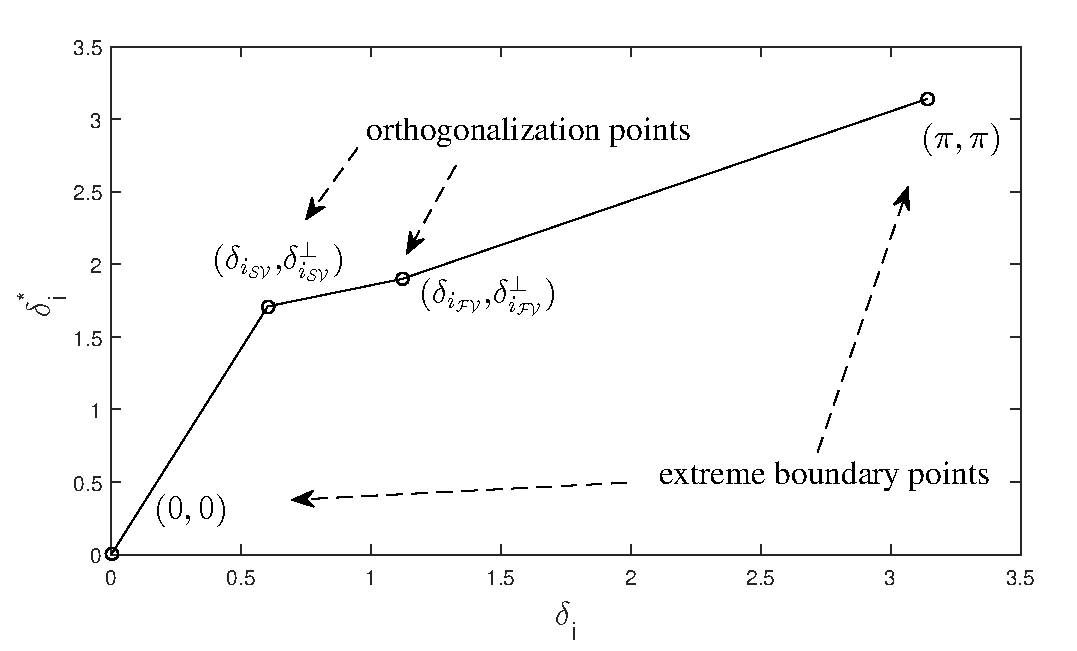
\includegraphics[scale=0.7]{Fig/simple_spline2.pdf}
\caption{\textcolor{black}{The simple mapping function for one angular dimension which maps the target points in the original space to the desired target points. Target points include the two extreme boundary points $(0,0)$, and $(\pi,\pi)$ as well as ($\delta_{i_{{\mathcal{SV}}}}$,$\delta^{\perp}_{i_{{\mathcal{SV}}}}$) and ($\delta_{i_{{\mathcal{FV}}}}$,$\delta^{\perp}_{i_{{\mathcal{FV}}}}$) to yield the desired mapping.} }%\textcolor{red}{add (0,0) and the label target and extreme boundary points to the figure.}}
%figure;plot([0,close,1.12,pi], [0,closed,1.9,pi],'-ko')
\label{fig:simple_spline}
\end{figure}

\section{Optimized Mapping Function}

The mapping function in Fig.\ref{fig:simple_spline} exhibits the two desired properties of monotonicity and continuity for an ideal mapping function $f_i$. However, this simple piecewise linear mapping function suffers from some drawbacks. Firstly, the function is not differentiable at the \textcolor{black}{orthogonalization} points ($\delta_{i_{{\mathcal{SV}}}}$,$\delta^{\perp}_{i_{{\mathcal{SV}}}}$) and ($\delta_{i_{{\mathcal{FV}}}}$,$\delta^{\perp}_{i_{{\mathcal{FV}}}}$), which can lead to severe cluster deformation. Secondly, the mapping function is applied to the angular dimensions, the discontinuity of the derivative of  %linearity of each spline in [RZ: I don't think, linearity causes this distortion.
the function can cause the convex-clusters to be mapped into non-convex clusters in the Cartesian coordinate system. In order to avoid deformations and to preserve maximal similarity with the original clustering geometry, it is desired to use a more linear functions with continuous derivatives. Also, in order to provide maximal separation among clusters and to concentrate clusters into disjoint non-overlapping clusters, it is beneficial to map the regions between two target points into a region with equal or even smaller range in the Cartesian coordinate system. In other words, it is desired to keep the samples close to the centroids in the mapped space as much as possible. This property is achieved by using nonlinear functions. However, there is a trade-off between the level of concentration and the linearity, which needs to be carefully addressed.  In order to avoid deformation while providing maximal separation, an optimized mapping function is proposed in this section.

In order to accommodate satisfy the above-mentioned requirements, it is desired to find a function, which satisfies the following mathematical conditions:

\begin{itemize}
\item the function is differentiable everywhere (continuous first derivative);
\item the derivative of the function is small at the target points, which correspond to the centroids of clusters in the original and transformed space, i.e. $\delta_{i_{{\mathcal{SV}}}}$ and $\delta_{i_{{\mathcal{FV}}}}$ in Fig. \ref{fig:optimized_p};
\item the derivative of the function is large at the boundaries of two regions (\textcolor{black}{point $(\epsilon_{i_{{\mathcal{SV}}}},\epsilon^{\perp}_{i_{{\mathcal{SV}}}})$ in Fig. \ref{fig:optimized_p})};
\end{itemize}


Therefore, we propose to use the basic function $p$ with adjustable parameters, which satisfies the aforementioned conditions. %\textcolor{red}{why you call it basis function. Basis function has a different meaning in linear analysis. I suggest you use the term basic function with adjustable parameters.} 
Each target point is associated with a basic function. 
The function $p$ is composed of two constitutive functions: $h(x)$ and $g(x)$, \textcolor{black}{respectively defined in two regions: i) from the target point to the upper boundary point, ii) from the lower boundary point to the next target point. }% [RZ: show h(x) and g(x) in Fig. 1.3.]. }
Before defining the two functions $h(x)$ and $g(x)$, we need to define the boundaries between two consecutive target points  ($\delta_{i_{{\mathcal{SV}}}}$,$\delta^{\perp}_{i_{{\mathcal{SV}}}}$) and ($\delta_{i_{{\mathcal{FV}}}}$,$\delta^{\perp}_{i_{{\mathcal{FV}}}}$), in which these functions are defined.% (i.g. $\epsilon_XXXX$). 
We simply choose the midpoint as the boundary points. For instance, we have $\epsilon=(\delta_1+\delta_2)/2$ %[RZ:Write the correct equation] 
as stated in Eq. \ref{eq:midpoint}.
The lower and upper boundary points are noted respectively as ($\gamma$,$\gamma^{\perp}$) and ($\epsilon$,$\epsilon^{\perp}$). To ensure the continuity of the mapping function $f$, the boundaries and target points should satisfy:
 
%The boundaries that each function activates are decided by target points ($\delta_{i_{{\mathcal{SV}}}}$,$\delta^{\perp}_{i_{{\mathcal{SV}}}}$) and ($\delta_{i_{{\mathcal{FV}}}}$,$\delta^{\perp}_{i_{{\mathcal{FV}}}}$) along with the mid-points between the target points. The lower boundary mid points are noted as ($\gamma$,$\gamma^{\perp}$). The upper boundary mid points are noted as ($\epsilon$,$\epsilon^{\perp}$). To ensure the continuity of the mapping function $f$, the boundaries and target points satisfy:

\begin{align}
\label{eq:midpoint}
\begin{aligned}
(\epsilon_{i_{{\mathcal{SV}}}},\epsilon^{\perp}_{i_{{\mathcal{SV}}}}) &=
(\gamma_{i_{{\mathcal{FV}}}},\gamma^{\perp}_{i_{{\mathcal{FV}}}}) &=
(\frac{\delta_{i_{{\mathcal{SV}}}} + \delta_{i_{{\mathcal{FV}}}}}{2}, \frac{\delta^{\perp}_{i_{{\mathcal{SV}}}} + \delta^{\perp}_{i_{{\mathcal{FV}}}}}{2})
\end{aligned}
\end{align}

The two piece-wise functions $h(x;\alpha,\epsilon,\epsilon^{\perp},\delta,\delta^{\perp})$ and $g(x;\alpha,\gamma,\gamma^{\perp},\delta,\delta^{\perp})$ are \textcolor{black}{the inverse of logit function} defined as follows:%\textcolor{red}{use the correct name: the inverse of logit/sigmoid function} as follows:

\begin{align}\label{eq:basicfunctions}
K_h &= \frac{\epsilon^{\perp}-\delta^{\perp}}{e^{\alpha(\epsilon-\delta,0)^{+}}-1}\\ \nonumber
h(x;\alpha,\epsilon,\epsilon^{\perp},\delta,\delta^{\perp}) &= K_h[e^{\alpha(x-\delta,0)^{+}}-1] + \delta^{\perp}
\end{align}
\begin{align}
K_g &= \frac{\gamma^{\perp}-\delta^{\perp}}{e^{\alpha(-\gamma+\delta,0)^{+}}-1}\\ \nonumber
g(x;\alpha,\gamma,\gamma^{\perp},\delta,\delta^{\perp}) &= K_g[e^{\alpha(\delta-x,0)^{+}}-1] + \delta^{\perp}
\end{align}

%\fbox{RZ: revised up to here}.

%\textcolor{red}{RZ: 1-include parameters in the function definitions: $h(x;\alpha,\epsilon, ....)$. 2-check functions, there are some typos like using different parameters in the denominator and nominator.}

In order to investigate the satisfaction of the above-mentioned conditions, we first verify that these functions pass through the target points. \textcolor{black}{More specifically, $g()$ should pass through points $(\gamma_{i},\gamma^{\perp}_{i}),~(\delta_{i}$,$\delta^{\perp}_{i})$ 
and $h()$ pass through $(\epsilon_{i},\epsilon^{\perp}_{i})$,  ($\delta_{i}$,$\delta^{\perp}_{i}$)} % and ($\delta_{i_{{\mathcal{FV}}}}$,$\delta^{\perp}_{i_{{\mathcal{FV}}}}$).

\begin{figure}[t]
\centering
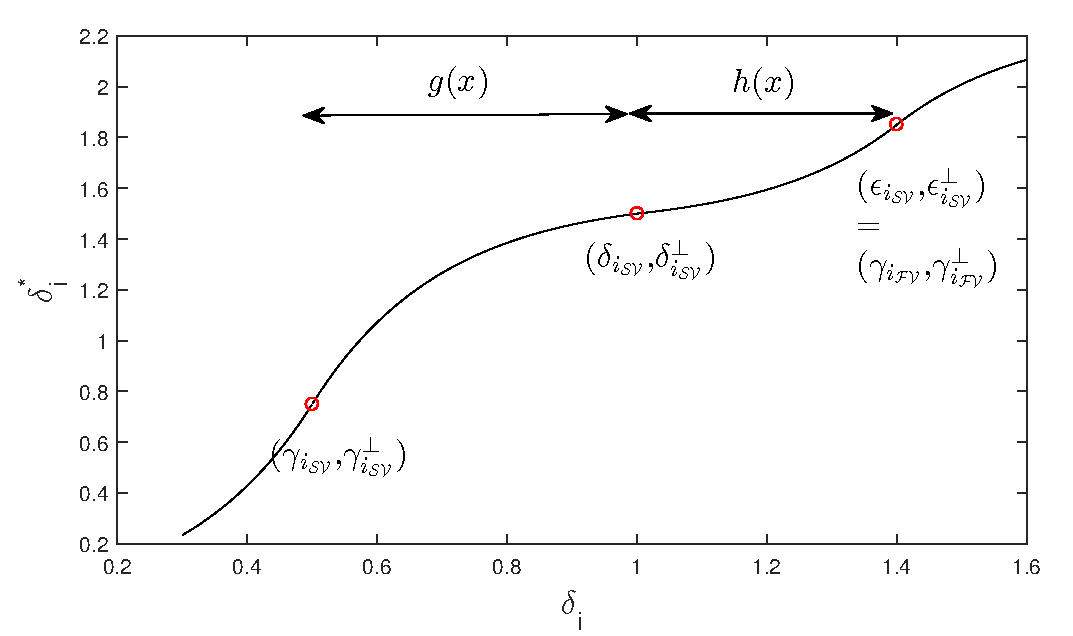
\includegraphics[scale=.7]{Fig/optimized_single_v2_croped.pdf}
\caption{Optimized Piece-wise Interpolated Function $p$.} %\textcolor{red}{I understand this figure, but is also misleading since the target points are at two ends and the boundary is in middle (the opposite is better). To solve this issue you can plot two adjacent regions and use tags and labels to show the target points $\delta$ and edge nodes/boundary nodes $\epsilon$}.}
\label{fig:optimized_p}
\end{figure}

\textcolor{black}{Once, we confirm that that the basic function $h(x)$ has the desired properties, we fit this function with appropriate parameters to all regions. The final function is a smooth and continuous function, which passes through all target points ($\delta_{i_{{\mathcal{SV}}}}$,$\delta^{\perp}_{i_{{\mathcal{SV}}}}$), ($\delta_{i_{{\mathcal{FV}}}}$,$\delta^{\perp}_{i_{{\mathcal{FV}}}}$) as well as the two extreme boundary points as shown in Fig.\ref{fig:optimized_map}.}

%To demonstrate this process, we first apply $p$ on two target points ($\delta_{i_{{\mathcal{SV}}}}$,$\delta^{\perp}_{i_{{\mathcal{SV}}}}$) and ($\delta_{i_{{\mathcal{FV}}}}$,$\delta^{\perp}_{i_{{\mathcal{FV}}}}$). This will result in a smooth curve as shown in Fig.\ref{fig:optimized_p}



%Therefore, if we apply the piecewise interpolate function $p$ at all four target points: ($\delta_{i_{{\mathcal{SV}}}}$,$\delta^{\perp}_{i_{{\mathcal{SV}}}}$), ($\delta_{i_{{\mathcal{FV}}}}$,$\delta^{\perp}_{i_{{\mathcal{FV}}}}$) and two boundary points of angular dimension, the final result is shown in Fig.\ref{fig:optimized_map}

\begin{figure}[t]
\centering
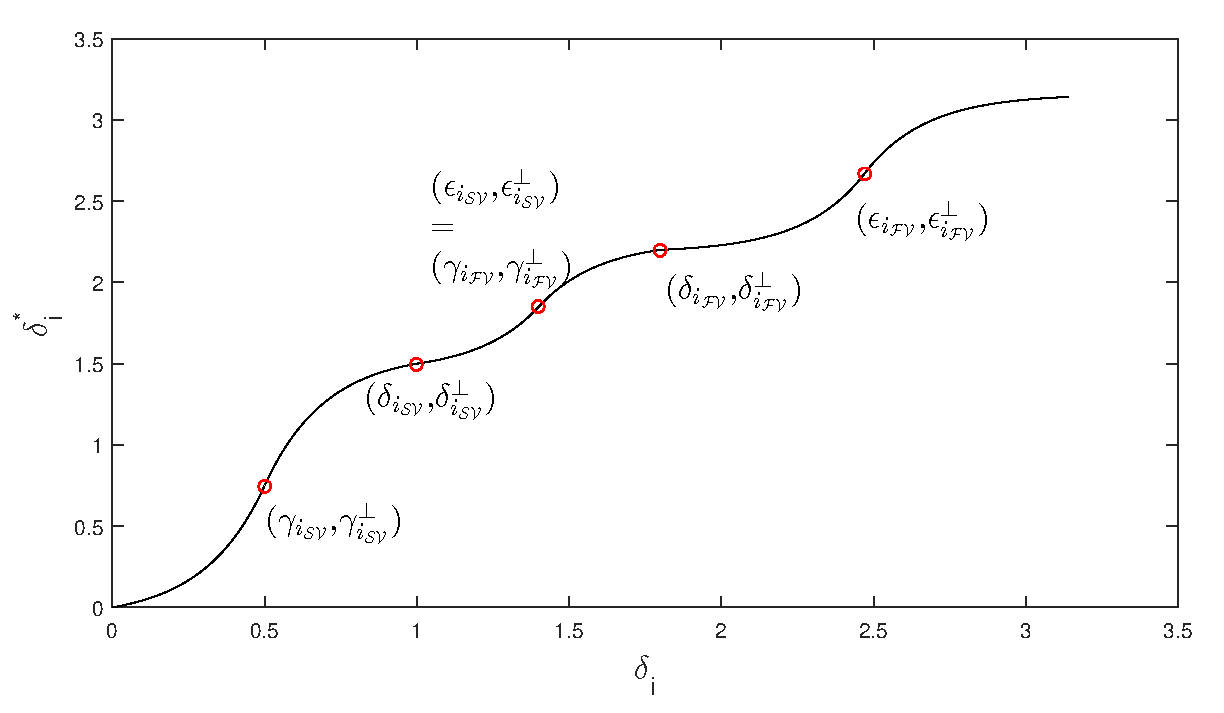
\includegraphics[scale=.7]{Fig/optimized_mapping_f.pdf}
\caption{Optimized Mapping Function $f$.}
\label{fig:optimized_map}
\end{figure}

In the training process, \textcolor{black}{data samples with abnormal labels belonging to all patients in DS1 and the personalized normal cluster for one patient are used to determine the mapping function for one corresponding patient. In the predicting process, the hyper-the the feature vector of new ECG sample in the spherical coordinate system is calculated and the mapping function is applied on its hyper-spherical coordinates to yield the transformed feature vector. After this step, we calculate the transformed data samples in the Cartesian coordinate system, which further fed into the personalized classification stage defined by Eq. \ref{eq:personal_discrim} to generate the corresponding type of \textit{yellow alarm}.} %\textcolor{red}{RZ: later make sure to use a consistent notation for equations Eq. or Equi. with or without parentheses.}%abnormal data from DS1 and personalized normal cluster are used to determine the mapping function. In the predicting process, the hyper-spherical coordinate of a new ECG sample is calculated and the mapping function is applied on its hyper-spherical coordinate. After this step, we calculate the Cartesian coordinate of the transformed data. This final result in Cartesian coordinate is then fed into Eq. \ref{eq:personal_discrim} to generate the corresponding type of yellow alarm.



\section{Experimental Results}\label{sec:result_spatial}

In this section, the performance of the proposed method is evaluated in terms of two aspects. We first analyze the classification performance of the system and then present the comparative results with respect to other representative ECG classifiers. Furthermore, the classification results are partitioned into two sets:  red alarms generated by the global classifier and the final labels by combining the yellow and red alarms. In this way, the impact of personalized classifier on the final labels can be revealed. Finally, the prediction power of the proposed method in terms of providing precaution hints for upcoming red alarms is evaluated.

\subsection{Classification Performance}

The experimental results are assessed in terms of classification performance of 4 AAMI ECG classes using the test subset of MITBIH Arrhythmia DS2. Originally, DS2 contains 15357 samples after feature extraction. While training the personalized classifier, the first 20\% of the normal samples serve as initialization set for the personalized dynamic normal cluster. \textcolor{black}{Therefore, we exclude the first 20\% of normal samples from each record since they are already included in the training process.} Consequently, the actual test set contains 12414 samples in total consisting of 10105 type-N, 1702 type-V, 508 type-S and 99 type-F samples.

To present the result, we select the weighted k-Nearest Neighbors method with $k=10$ as our choice of global classifier because it is \textcolor{black}{one of the low-complexity methods with a relatively good classification accuracy\cite{hechenbichler2004weighted}. }%comparatively simple and representative among low complexity models. 
The parameter $\alpha$, \textcolor{black}{used in Eq. \ref{eq:basicfunctions}} in the deviation detection module is set to 1 for test purpose. 
%\textcolor{red}{if there are more parameters you can define here.}


Table \ref{table:classification_cumu} summarizes the cumulated confusion matrix for all records in the test set. In order to compare the result of global classifier (red alarms) and combined results (final labels including both red and \textit{yellow alarms}), the sample numbers are presented in the following format: $final~label(primary~label~by~global~ classifier)$. In order to measure the classification performance, we adopt three metrics: accuracy($Ac$), sensitivity($Se$), specificity($Sp$), as proposed in \cite{Hu_et_al,deChazal2006,ince2009generic}. All three metrics are calculated based on the true positive $TP$, false positive $FP$, false negative $FN$ and true negative $TN$ in a binary confusion matrix, \textcolor{black}{where one class is the specific abnormality class and all other abnormality and normal classes combined into one class}. Therefore all four metrics are calculated for each class by converting the 4x4 matrix to a 2x2 matrix.

\begin{table}[t]
	\centering
	\caption{Cumulated Confusion Matrix for All Records in DS2. \textcolor{black}{The numbers are $final~label(primary~label~by~global~ classifier)$}.}
	\vspace{-0.05in}
	\begin{tabular}{|l|l|c|c|c|c|}
		\hline 
		&  \multicolumn{4}{c}{Ground Truth} &\\ 
        \hline
		\multirow{5}{*}{Result} &  & N & V & S & F  \\\cline{2-6}
		& N & 9255(10076)& 21(38) & 72(90) & 1(5) \\\cline{2-6} 
		&V & 657(22) & 1678(1663) & 8(2) & 9(7)  \\\cline{2-6}
		&S & 71(6) & 3(1) & 417(416) & 0(0)  \\\cline{2-6}
        &F& 122(1) & 0(0) & 11(0) & 89(87)  \\\hline
	\end{tabular}
	\label{table:classification_cumu} 
	\vspace{-0.15in}
\end{table}

While cumulative classification results are demonstrated in Table \ref{table:classification_cumu}, the robustness of the proposed method should be evaluated based on the performance variation over 22 test records in DS2. Further, medians and IQRs (interquartile range) for each metric and each class are included in Table \ref{table:variation} to represent the robustness of proposed methods. \textcolor{black}{The robustness of the system is assesed in terms of the variation between the performance of different types. The system is more robust if this variation is lower.} 
In Table \ref{table:variation}, we observe that among all abnormality classes,  %\textcolor{red}{It is ok to use abnormal class, but since we used abnormality class, better to be consistent throughout the write-up.}, 
the proposed method demonstrates a stable performance on class V but a lower stability for classes S and F.


\begin{table}[t]
\centering
\caption{Classification Performance and Within-Set Variation of Proposed System}
\label{table:variation}
\resizebox{\textwidth}{!}{
\begin{tabular}{|c|c|c|c|c|c|c|c|c|c|c|c|c|}
\hline
\multirow{2}{*}{statistics} & \multicolumn{3}{c|}{N}                  & \multicolumn{3}{c|}{V}                  & \multicolumn{3}{c|}{S}                  & \multicolumn{3}{c|}{F}                  \\ \cline{2-13} 
                            & \textit{Ac} & \textit{Se} & \textit{Sp} & \textit{Ac} & \textit{Se} & \textit{Sp} & \textit{Ac} & \textit{Se} & \textit{Sp} & \textit{Ac} & \textit{Se} & \textit{Sp} \\ \hline
cumulated                   & 92.4        & 91.59       & 95.93       & 94.38       & 98.59       & 93.71       & 98.67       & 82.09       & 99.38       & 98.85       & 89.9        & 98.92       \\ \hline
median                      & 94.45       & 92.21       & 95.42       & 96.17       & 99.55       & 95.71       & 99.38       & 80.65       & 99.84       & 99.11       & 90.91       & 99.11       \\ \hline
IQR                         & 6.33        & 10.08       & 11.91       & 5.17        & 1.64        & 8.62        & 1.76        & 19.35       & 0.61        & 1.58        & 23.33       & 1.49        \\ \hline
\end{tabular}}
\end{table}

As MITDB is widely used to verify ECG classifier performance, we compared the proposed system with five significant methods proposed in the literature. According to AAMI standards, the performance of ECG classification should be evaluated over the binary classifiers applied to \textit{Ventricular (V)} versus \textit{non-V}types and \textit{Supraventricular (S)} versus \textit{non-S} types. For methods proposed in the literature, the same evaluation metrics are commonly used applied to records from MITDB. To standardize the metrics, we select 11 ECG records which are common among all 5 methods and compare the median of each classification metrics over these 11 records. The comparison results are presented in Table \ref{table:classification_comp}. Generally speaking, the proposed method shows a higher sensitivity for both types V and S. Especially for type S, the proposed method shows an advantage over all three metrics compared to the five reference methods.


\begin{table}[tbp]
\centering
\caption{V and S classification performance compared with five algorithms in literature using 11 common records in MITDB}
\label{table:classification_comp}
\begin{tabular}{|c|c|c|c|c|c|c|}
\hline
\multirow{2}{*}{Methods} & \multicolumn{3}{c|}{V} & \multicolumn{3}{c|}{S} \\ \cline{2-7} 
                         & Ac     & Se     & Sp     & Ac      & Se     & Sp     \\ \hline
Proposed                 & 96.6   & 98.2   & 92.4   & 98.63   & 88.89  & 99.41  \\ \hline
Hu \textit{et al.}\cite{Hu_et_al}     & 94.8   & 78.9   & 96.8   & N/A     & N/A    & N/A    \\ \hline
de Chazal \textit{et al.}\cite{autofs}  & 96.4   & 77.5   & N/A    & N/A     & N/A    & N/A    \\ \hline
Jiang and Kong \cite{bbnn}    & 98.8   & 78.9   & 96.8   & 97.5    & 74.9   & 98.8   \\ \hline
Ince \textit{et al.} \cite{ince2009generic}    & 97.9   & 90.3   & 98.8   & 96.1    & 81.8   & 98.5   \\ \hline
Kiranyaz \textit{et al.}\cite{Kiranyaz}         & 98.9   & 95.9   & 99.4   & 96.4    & 68.8   & 99.5   \\ \hline
\end{tabular}
\end{table}

\subsection{Prediction Performance}

As an important feature of the proposed method, \textit{yellow alarms} triggered by the personalized classifier indicate a higher probability of observing subsequent abnormalities. In order to verify this functionality, all beats following a \textit{yellow alarm} of a specific type is investigated to asses the chance of upcoming red alarms of different types. This process is repeated for \textit{yellow alarms} of all types. We only account for the first abnormality type which occurs after the \textit{yellow alarm}. As we used confusion matrix to evaluate the classification accuracy, the performance of prediction can be summarized by a confusion matrix with the 3 abnormal types. Probabilities of observing a certain type of abnormal beat after a \textit{yellow alarm} is calculated using the prediction confusion matrix and compared to the prior probability of observing the abnormality of the same type. This process is formulated in the following two equations:

\begin{align}
\nonumber 
&P(\hat{y}_{k+i}=X_r|\hat{y}_{k}=X_y)=\frac{\text{\# of $y_{k+i}=X$ after $\hat{y}_k=X_y$}}{\text{\# of true alarms after $\hat{y}_k=X_y$}} \\
&P(\hat{y}_{k+i}=X_r)=\frac{\text{\# of true alarm of type $X$ ($y_{k}=X$)}}{\text{\# of all true alarms}} 
\end{align}

The prediction power of each abnormality type is evaluated by comparing $P(\hat{y}_{k+i}=X_r|\hat{y}_{k}=X_y)$ and $P(\hat{y}_{k+i}=X_r)$. A shown in Table \ref{table:pred}, the probability of observing a certain type of abnormalities after a \textit{yellow alarm} is higher than its prior probability and this fact is consistent for abnormality types. For example, without knowing the type of a \textit{yellow alarm}, the probability of observing a type $V$ sample is 71.54\%, while the probability of observing a type $V$ sample after observing a \textit{yellow alarm} of a type $V$ is 77.45\% ($5.91\%$ higher than the prior probability). The improvement are consistent among all three types of abnormalities but the system shows a stronger prediction power for type $S$. 

\begin{table}[t]
\centering
\caption{predictive probability versus prior probability without windowing}
\label{table:pred}
\begin{tabular}{|c|l|l|l|l||l|l|l|}
\hline
\multicolumn{2}{|l|}{\multirow{2}{*}{}} & \multicolumn{3}{m{8em}|}{\# of predicted ground truth} & \multicolumn{3}{m{8em}|}{\% of predicted ground truth} \\ \cline{3-8} 
\multicolumn{2}{|l|}{}                  & V               & S               & F             & V               & S               & F             \\ \hline
\multirow{3}{2.5em}{\textit{yellow} alarm}    & V    & 467             & 122              & 14            & \textbf{77.45}  & 20.23           & 2.32          \\ \cline{2-8} 
                                 & S    & 36              & 15              & 0             & 70.59           & \textbf{28.41}  & 0             \\ \cline{2-8} 
                                 & F    & 40              & 60              & 5             & 38.10           & 57.14           & \textbf{4.76} \\ \hline
\multicolumn{2}{|c|}{total}             & 543             & 197             & 19            & \textbf{71.54}  & \textbf{25.96}  & \textbf{2.50} \\ \hline
\end{tabular}
\end{table}

\textcolor{black}{In the above analysis we consider the first subsequent red alarm regardless of the time passes since the preceding \textit{yellow alarm}.} In order to study the impact of the timing window (the time between the \textit{yellow alarm} and the subsequent red alarm), we also studied a window of 10 consecutive samples following a \textit{yellow alarm}. Similarly, the prior and posterior probabilities are compared to evaluate the performance of the prediction capacity as shown in Table.\ref{table:pred10}. %\textcolor{red}{RZ: We can generate more insightful results for the journal paper, like a curve to show the prediction improvement vs time, etc...}


\begin{table}[t]
\centering
\caption{predictive probability versus prior probability within 10 beats' window}
\label{table:pred10}
\begin{tabular}{|c|l|l|l|l||l|l|l|}
\hline
\multicolumn{2}{|l|}{\multirow{2}{*}{}} & \multicolumn{3}{m{8em}|}{\# of predicted ground truth} & \multicolumn{3}{m{8em}|}{\% of predicted ground truth} \\ \cline{3-8} 
\multicolumn{2}{|l|}{}                  & V               & S               & F             & V               & S               & F             \\ \hline
\multirow{3}{2.5em}{\textit{yellow} alarm}    & V    & 290             & 85              & 12            & \textbf{74.94}  & 21.96           & 3.10          \\ \cline{2-8} 
                                 & S    & 22              & 13              & 0             & 62.86           & \textbf{37.14}  & 0             \\ \cline{2-8} 
                                 & F    & 29              & 37              & 6             & 40.28           & 51.39           & \textbf{8.33} \\ \hline
\multicolumn{2}{|c|}{total}             & 341             & 135             & 18            & \textbf{69.03}  & \textbf{27.32}  & \textbf{3.64} \\ \hline
\end{tabular}
\end{table}

Compared with the result without windowing, the prediction performance within a 10-sample window shows that the proposed algorithm can better predict the occurrence of abnormalities if a certain timing window is used. Especially for type S, the probability of observing a sample of type S within 10 beats after a \textit{yellow alarm} of type S is 27.32\%, %while given that the \textit{yellow alarm} is type S, 
i.e. the posterior probability rises to 37.14\%. With almost 10\% increase, it is proved that the \textit{yellow alarm} types are informative. The results shows that same improvements are made within the 10-sample window as well. In general, the predicting performance are promising, indicating the efficiency of personalized classifier and deviation analysis. We believe that this concept is worthy of further more in-depth studies for different physiological signals.




\section{Summary of Contributions}
%We have such a section in Chapter 3. Add a short section here and at the end of Chapter 2 for consistency. Make tis section quite short: one or two para at most.

\textcolor{black}{In this chapter, we proposed a novel deterministic spatial transformation. The purpose is to reshape the original feature space so that the clusters in the transformed feature space demonstrate symmetry and low within-cluster variance. This method is more tractable and analytical than the method proposed in chapter 3.}

\textcolor{black}{The method utilizes hyper-spherical coordinate and orthogonalization to determine the parameters in basic functions of mapping function. The mapping function is deterministic. We applied this method on test dataset MITDB DS2 and obtained promising results. Both classification and prediction performance of the proposed method are analyzed in this chapter. The algorithm has been proven to be efficient in classifying samples and predicting upcoming abnormalities as well. }
